\newpage
\begin{center}
    \textbf{\large 1. ОБЗОР СОВРЕМЕННЫХ ТЕХНОЛОГИЙ И ПРИНЦИПОВ СОЗДАНИЯ АВТОМАТИЗИРОВАННЫХ ИНФОРМАЦИОННЫХ СИСТЕМ}
\end{center}
\refstepcounter{chapter}
\addcontentsline{toc}{chapter}{1. ОБЗОР СОВРЕМЕННЫХ ТЕХНОЛОГИЙ И ПРИНЦИПОВ СОЗДАНИЯ АВТОМАТИЗИРОВАННЫХ ИНФОРМАЦИОННЫХ СИСТЕМ}


\section{Современные технологии, используемые для создания автоматизированных информационных систем}

\textbf{Автоматизированные информационные системы (АИС)} - это комплекс программных и аппаратных средств,
предназначенных для автоматизации различных задач в организациях и предприятиях.
С развитием технологий и появлением новых методов обработки данных,
АИС стали все более востребованными и широко используемыми.
В данной главе рассматриваются основные технологии и принципы, используемые при создании АИС.

\textbf{Базы данных (БД)} - это средства хранения и организации данных,
обеспечивающие эффективный доступ к ним. Существует множество различных систем управления базами данных (СУБД),
таких как MySQL, PostgreSQL, Oracle, MS SQL Server и др.
Каждая СУБД имеет свои преимущества и недостатки, и выбор конкретной СУБД зависит от требований к системе.

\textbf{Доменное имя} - это уникальное имя, используемое для идентификации компьютера, сервера или другого устройства, подключенного к Интернету.
Оно представляет собой читаемое для людей название, которое соответствует числовому IP-адресу,
который используется компьютерами для идентификации друг друга в сети.

\textbf{Клиент} - это устройство или приложение, которое запрашивает информацию у другого устройства, называемого сервером. 
Клиент может быть любым устройством, например, компьютером, мобильным устройством или планшетом, 
которое подключено к сети Интернет или локальной сети. 
Клиентское устройство обычно используется для ввода данных или запросов, 
которые передаются на сервер для обработки.

\textbf{Сервер} - это компьютер или другое устройство, которое предоставляет информацию клиентским устройствам. 
Сервер может выполнять различные задачи, такие как обработка запросов клиентов, 
хранение данных, предоставление доступа к сети Интернет, управление ресурсами сети и многое другое.
Сервер может обслуживать множество клиентов одновременно, предоставляя им доступ к различным ресурсам.

В общем случае, клиент и сервер образуют взаимодействующие компоненты,
которые работают совместно для выполнения различных задач в сети.
Клиент отправляет запросы на сервер, а сервер обрабатывает эти запросы и отвечает клиенту.
Коммуникация между клиентом и сервером может происходить по различным протоколам, например, HTTP, FTP, SMTP и т.д.

\textbf{Мобильное приложение} - это программа, которая разработана для работы на мобильных устройствах,
таких как смартфоны и планшеты. Они обычно загружаются из центра приложений на мобильном устройстве,
таком как App Store или Google Play, и устанавливаются на устройство.
Мобильные приложения могут выполнять различные задачи, включая игры, социальные сети,
продуктивные инструменты, торговые платформы, и т.д.
В том числе, мобильные приложения могут быть использованы для доступа участников учебного процесса к расписанию.

Мобильные приложения могут быть созданы для разных операционных систем, 
таких как iOS, Android, Windows Mobile и т.д.
Каждая операционная система имеет свои собственные инструменты и языки программирования для создания мобильных приложений.
Например, для создания мобильных приложений для iOS,
нужно использовать язык программирования Swift или Objective-C, а для Android - Java или Kotlin.

Мобильные приложения имеют множество преимуществ перед другими типами программ.
Они могут использовать различные функции мобильных устройств, такие как камера, GPS, датчики, уведомления и т.д.,
чтобы создать более интуитивный и персонализированный пользовательский опыт.
Также мобильные приложения могут работать в автономном режиме, без подключения к Интернету,
что делает их более удобными для использования в путешествиях или в местах, где связь ограничена.

\textbf{Чат-бот} - это программа, которая может общаться с пользователем через интерфейс чата, 
похожий на тот, который используется в мессенджерах. 
Она может выполнять определенные задачи и предоставлять определенную информацию в ответ на запросы пользователя.

\textbf{ICS (iCalendar)} - это открытый стандарт, 
который определяет формат обмена календарными данными между различными приложениями и устройствами. 
Формат данных, используемый в iCalendar, позволяет описывать события, задачи, напоминания и другие элементы, 
связанные с управлением временем.

Файлы в формате ICS могут быть импортированы в календарные приложения, 
такие как Google Календарь, Microsoft Outlook, Apple iCal и другие, 
что позволяет пользователям синхронизировать свои расписания между различными устройствами и приложениями.

\textbf{API (Application Programming Interface)} - это набор правил, протоколов и инструментов, 
которые используются для создания программных приложений и позволяют им взаимодействовать с другими приложениями и системами. 
API предоставляет возможность разработчикам использовать функциональность и данные, 
предоставляемые другими приложениями или системами, 
без необходимости понимания внутренней работы их компонентов.

\textbf{GraphQL} - это язык запросов, разработанный Facebook для работы с API. 
Он позволяет клиентам запрашивать только те данные, которые им необходимы, и получать их в одном запросе. 
В отличие от REST API, где клиенты получают предопределенный набор данных, 
GraphQL предоставляет клиентам возможность выбирать конкретные поля и связи, 
которые им нужны, и получать только эти данные.
GraphQL имеет множество преимуществ по сравнению с REST API. 
Он позволяет более гибко и эффективно работать с данными, 
улучшает производительность и упрощает поддержку кода. Кроме того, 
GraphQL позволяет создавать более сложные запросы и связи между данными, 
что упрощает создание более мощных и гибких API.

\textbf{JSON} - это текстовый формат обмена данными, основанный на JavaScript.
Он используется для передачи данных между веб-приложениями и серверами.
JSON представляет собой набор пар ключ-значение, разделенных запятыми,
















\section{Влияние дальнодействия потенциала на фазовые диаграммы и плавление}

Понимание фазовых переходов в 2D-системах имеет большое значение в ряде областей, начиная с фотоники и электроники  и заканчивая новыми материалами и биотехнологиями, поскольку знание фазового поведения открывает путь к проектированию систем с желаемыми свойствами. 
Несмотря на многочисленные исследования, основные вопросы в данной области по-прежнему связаны с влиянием конкретного взаимодействия между отдельными частицами на их коллективное поведение. 
Для классических систем одной из простейших моделей, способных воспроизвести поведение веществ, включая газовую, жидкую и твердую фазы, является система Леннарда-Джонса (LJ). 
Модель LJ широко используется для анализа поведения молекулярных, белковых, полимерных, эмульсионных и коллоидных мягких веществ. 
Обобщенный LJ-потенциал (или LJn-m-потенциал, где индексы n и m отвечают за алгебраические ветви отталкивания и притяжения) является подходящей моделью для исследований, направленных на выявление эффектов отталкивания и притяжения в жидкостях, твердых телах и фазовых переходов между ними.

В настоящий момент установлено, что 2D-сценарии плавления зависят от мягкости отталкивания, обеспечивая микроскопические сценарии 2D-плавления, описываемые в работах~\cite{10.3367/ufne.2017.06.038161, 10.3367/ufne.2018.04.038417}, что доказывает теория Березинского-Костерлица-Таулесса-Гальперина-Нельсона-Янга (БКТГНЯ), согласно которой плавление происходит через два непрерывных перехода с промежуточной гексатической фазой с квазидальним ориентационным порядком и ближним трансляционным порядком~\cite{10.1088/0022-3719/6/7/010, 10.1103/physrevlett.41.121, 10.1103/physrevb.19.2457, 10.1103/physrevb.19.1855}, плавление через фазовый переход первого рода, двухстадийное плавление, включающее непрерывный (Березинский-Костерлиц-Таулесс, БКТ) кристаллогексатический фазовый переход и фазовый переход первого рода между гексатической фазой и изотропной жидкостью.
Второй и третий сценарии присущи системам с короткодействующим (жестким) отталкиванием, тогда как первый наблюдался при мягком отталкивании между частицами. 
Установлено, что мягкость отталкивания влияет на сценарии плавления, термодинамику и спектры возбуждения в монослойных системах. 
Однако известно, что роль притяжения в сценарии плавления монослойных систем остается систематически неизученной.

LJ-взаимодействия были одними из первых систем, попытки изучения которых предпринимались для понимания роли притяжения в плавлении. 
Тем не менее, многие опубликованные результаты, рассматривающие критическую точку и сценарий плавления для 2D-кристаллов LJ, не дают исчерпывающего ответа на роль притяжения в данных процессах.
Например, чтобы определить критическую температуру в зависимости от радиуса обрезки потенциала, было выполнено численное моделирование кривой пар-жидкость в ансамбле Гиббса, согласно ~\cite{10.1063/1.460477}.
О противоречивых сценариях плавления треугольного кристалла говорилось в ранних работах~\cite{10.1103/physrevlett.42.1632, 10.1063/1.436526, 10.1103/physrevlett.44.463, 10.1063/1.441901, 10.1103/physrevlett.52.449, 10.1103/physrevb.30.2755}, включая два непрерывных перехода с промежуточной гексатической фазой по теории БКТГНЯ~\cite{10.1103/physrevlett.42.1632} и переход первого рода~\cite{10.1063/1.436526, 10.1103/physrevlett.44.463, 10.1063/1.441901, 10.1103/physrevlett.52.449}.

Благодаря росту вычислительных возможностей моделирование больших систем ($\gtrsim 10^5$ частиц) дало новые результаты по двумерному плавлению кристаллов Леннарда-Джонса и связанных с ними систем.
Моделирование систем с последующим анализом их уравнения состояния и дальнодействующей асимптотики трансляционной корреляционной функции (которая точно обеспечивает предел устойчивости кристалла) позволило однозначно идентифицировать сценарии плавления. 
Например, об изменении сценария плавления говорилось в работе~\cite{10.1103/physreve.99.022145}, где авторы изучали двумерные системы частиц, взаимодействующих посредством обобщенного потенциала Леннарда-Джонса с различными ветвями отталкивания ($\propto 1/r ^{12}$ и $\propto 1/r^{64}$).
Выявлено, что сценарий реализуется через фазовые переходы первого рода при низких температурах и через два непрерывных перехода БКТ при высоких.
Раньше предполагалось, что LJ-система при высоких температурах близка к мягким отталкивающим дискам $1/r^{12}$, но такая экстраполяция на сценарий плавления противоречит результатам приведённого исследования~\cite{10.1103/physrevlett.114.035702}, согласно котррому мягкие диски $1/r^n$ с $n>6$ плавятся по третьему сценарию. 
Предполагалось, что петля Майера-Вуда, присущая переходу первого рода, исчезает при высоких температурах с увеличением размера системы. 
Однако объяснение эффекта конечно-размерным масштабированием кажется неубедительным: с увеличением размера системы петля должна сплющиваться и в конечном итоге приближаться к плато~\cite{10.1103/physreve.87.042134, 10.1103/physreve.59.2659}.

Было установлено, что при низких температурах, где преобладает роль притяжения, все системы плавятся по переходу первого рода за счет подавления гексатической фазы.
При высоких температурах LJ-диски плавятся по третьему сценарию, как и мягкие диски~\cite{10.1103/physrevlett.114.035702}.

Известно, что кристаллы LJ по сравнению с системой Морзе в~\cite{10.1103/physrevb.103.094107} плавятся по третьему сценарию при низких температурах. 
Данный вывод согласуется с~\cite{10.1103/physreve.99.022145}, но противоречит~\cite{10.1103/physrevlett.114.035702}. 
Сценарий БКТГНЯ при высоких температурах был поставлен под сомнение из-за кажущегося исчезновения петли Майера-Вуда, аналога петли Ван-дер-Ваальса в трехмерном случае.
Для мягких взаимодействий Морзе третий сценарий плавления наблюдается для всех температур, рассмотренных в~\cite{10.1103/physrevb.103.094107}, тогда как авторы исследования ожидали наблюдать сценарий БКТГНЯ при более высоких температурах.
Однако, с некоторыми параметрами мягкости потенциала уже при низких температурах, учитывая дальнодействующее притяжение, наблюдались два непрерывных перехода.

Роль притяжения можно проверить экспериментально в коллоидных системах, известных как модельные системы, демонстрирующих широкий спектр ``молекулярно-подобных'' явлений~\cite{book.fernandez, book.ivlev, 10.1016/0370-1573(94)90017-5, 10.1038/natrevmats.2015.11, 10.1039/c9sm01953g}, в частности кристаллизация и плавление~\cite{10.1126/science.1112399, 10.1039/c2sm26473k, 10.1103/physrevlett.82.2721, 10.1103/physrevlett.85.3656, 10.1103/physrevlett.118.088003, 10.1039/c2sm27654b, 10.1126/science.1224763, 10.1038/s41598-021-97124-7}.

Эти коллективные явления визуализируются в реальном времени с пространственным разрешением отдельных частиц.
Дальнодействующее дипольное притяжение $\propto 1/r^3$ в коллоидных системах индуцируется и контролируется in situ с помощью вращающегося в плоскости магнитного поля~\cite{10.1088/0034-4885/76/12/126601, 10.1039/c3sm50306b, 10.1039/c3sm27620a, 10.1103/physrevmaterials.2.025602} или электрического~\cite{10.1088/1367-2630/8/11/267, 10.1063/1.3115641, 10.1021/la2014804, 10.1021/la500178b, 10.1039/c1sm06414b, 10.1038/s41598-017-14001-y} поля.
Используя конически вращающиеся магнитные или электрические поля с магическими углами, может быть создано Ван-Дер-Ваальсово притяжение $\propto 1/r^6$ с "магическими" полями~\cite{10.1021/la500896e, 10.1103/physrevlett.103.228301}.
В последнее время настраиваемые взаимодействия были достигнуты за счет использования пространственных годографов внешнего электрического или магнитного поля~\cite{10.1039/d0sm01046d}, проектирования внутренней структуры~\cite{10.1063/5.0055566} и геометрии~\cite{10.1063/5.0060705} коллоидных частиц.

Моделирование систем частиц производится с помощью обобщенного потенциала Леннарда-Джонса (LJn-m):

\begin{equation}
U_{n m}(r)=\frac{\epsilon}{n-m}\left[m\left(\frac{\sigma}{r}\right)^{n}-n\left(\frac{\sigma}{r}\right)^{m}\right]
\label{LJnm}
\end{equation}

где $n$ и $m$ — индексы отталкивающей и притягивающей ветвей соответственно, а $\sigma$ и $\epsilon$ — характерная длина взаимодействия и глубина потенциальной ямы.
Потенциал имеет минимум $-\epsilon$ при $r/\sigma=1$.
В дальнейшем нормируются расстояния и энергии на $\sigma$ и $\epsilon$ соответственно и рассматриваются частицы одинаковой массы $m=1$.

Вблизи критической температуры вычисление плотностей газа и конденсата становится затруднительным из-за растущих флуктуаций плотности в системе.
Тем не менее, следующим образом может быть рассчитано положение критической точки на фазовой диаграмме путем аппроксимации конденсированных и газовых бинодальных ветвей вблизи критической точки:
\begin{equation}
    n_{c}-n_{g} \simeq A \tau^{\beta}, \quad n_{c}+n_{g} \simeq a \tau+2 n_{\mathrm{CP}},
\label{MACR-eq4}
\end{equation}
где $\tau=T_{\mathrm{CP}}-T$, $T_{\mathrm{CP}}$ и $n_{\mathrm{CP}}$ -- это температура и 
плотность в критической точке соответственно, $\beta$ -- критический индекс, $A$ и $a$ являются параметрами, которые должны быть получены из аппроксимации $n_{\mathrm{CP}}$ и $T_{\mathrm{CP}}$.
Критический индекс $\beta$ зависит от класса универсальности системы, определяемого межчастичным взаимодействием~\cite{10.1103/physrevlett.89.025703}.

Результаты для бинодали конденсат-газ, полученные с помощью метода фазовой идентификации и уравнения состояния, представлены на рисунке~\ref{nmp}.
Цветными кругами обозначены плотности газа, конденсата и их среднее значение для каждого рассмотренного потенциала. 
Сплошные серые линии — области, в которых использовали аппроксимацию для получения значений критической точки с помощью уравнений~\ref{MACR-eq4}. 
Серыми пунктирными линиями показана экстраполяция фазовой диаграммы до критических точек, обозначенных цветными звездочками.

\begin{figure}[!h]
\begin{center}
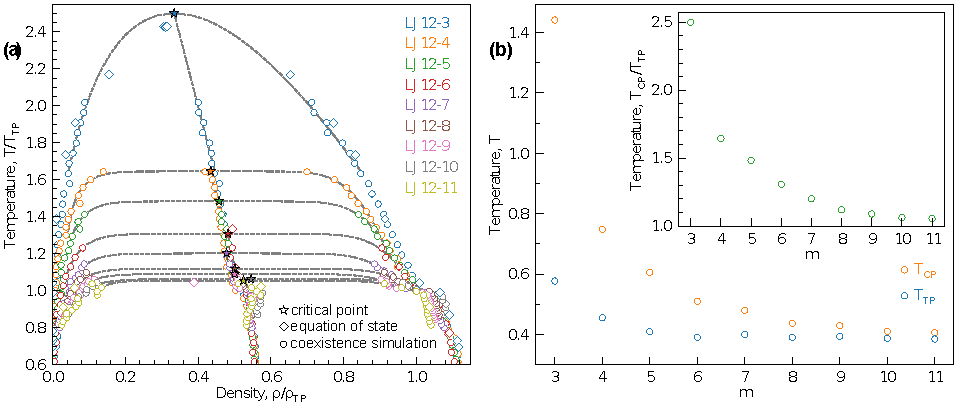
\includegraphics[width=\textwidth]{NMP-Figure4.pdf}
\caption{Влияние диапазона притяжения на область сосуществования жидкость-газ на фазовой диаграмме: (a) бинодали конденсат-газ для разных потенциалов LJ12-m; круги — точки бинодали и медианы (полученные методом фазовой идентификации), ромбы — точки, полученные из уравнения состояния, серые линии — аппроксимации бинодали, звездочками обозначены критические точки.
	(b) Зависимости тройной и критической температур от индекса притяжения m для взаимодействия LJ12-m, отношение $T_{CP}$/$T_{TP}$ показано на вставке.}
\label{nmp}
\end{center}
\end{figure}

Падение диапазона притяжения снижает критическую температуру, а также отношение между температурами критической и тройной точек, как показано на рисунке~\ref{nmp}(b) и соответствующей вставке.
С увеличением $m$ двухфазная область сужается в сторону меньших плотностей, а отношение между критической и тройной температурами приближается к единице.
Для LJ-взаимодействия ($m = 6$) полученная критическая температура $T_c=(0,51 . . . 0,52)$ (в зависимости от метода оценки) согласуется с предыдущими результатами $T_c = 0.515 \pm 0.002$  для LJ-потенциала.

В данном разделе был проведен обзор эволюции фазовых диаграмм и сценариев плавления двумерных систем частиц, взаимодействующих через обобщенный потенциал Леннарда-Джонса с разным диапазоном притяжения, в то время как ветвь отталкивания зафиксирована.

Переход жидкость-газ изучается с помощью анализа уравнения состояния и метода фазовой идентификации.
Результаты, полученные двумя упомянутыми методами, хорошо согласуются друг с другом.
Плавление при высоких температурах и высоких плотностях в системе мягких сфер $1/r_{12}$ происходит согласно третьему сценарию. 
Однако при низких температурах плавления в системах с $m = 6$, $9$ и $11$ было выявлено изменение сценария плавления от третьего к переходу первого порядка (без гексатической фазы).
Обнаружено, что температура изменения сценариев смещается в сторону более низких температур с увеличением диапазона притяжения, что соответствует уменьшению $m$. 
Анализ случая $m = 9 (LJ12-9)$  показал, что для короткодействующего притяжения наблюдается третий сценарий плавления.

Однако на данный момент не существует теории, которая предсказывала бы поведение транспортных свойств и коллективных возбуждений в зависимости от дальнодействия притяжения.
В связи с этим формулируются следующие цели и задачи настоящей работы.

\section{Цели и задачи магистерской работы}

\textbf{Цель работы} -- установить связь дальнодействия притяжения потенциала взаимодействия и спектров возбуждений с транспортными свойствами жидкостей, а также влияние на скорость нуклеации.

\textbf{Задачи работы:}
\begin{enumerate}
    \item Расчет фазовых диаграмм для 2D и 3D систем частиц, взаимодействующих посредством обобщенного потенциала Леннарда-Джонса с различными степенями притяжения.
    \item Адаптация метода кластеризации данных DBSCAN для изучения молекулярных систем и его сравнение с другими методами.
    \item Расчет и анализ транспортных свойств и коллективных возбуждений на жидкостных бинодалях.
    \item Применение нового метода распознавания фаз для изучения скорости нуклеации в переохлажденных системах Леннарда-Джонса с различным дальнодействием притяжения.
\end{enumerate}
